\documentclass[a3 paper]{article}
%\usepackage[textwidth=8cm,textheight=5cm]{geometry}
\usepackage{paracol}
\usepackage{pdflscape}
\usepackage{kantlipsum}
\usepackage{lipsum}
\usepackage[margin=.5in]{geometry}

\usepackage[utf8]{inputenc}
\usepackage[TS1,T1]{fontenc}
%\usepackage{fourier, heuristica}
\usepackage{array, booktabs}
\usepackage{graphicx}
\usepackage[x11names,table]{xcolor}
\usepackage{caption}
\DeclareCaptionFont{blue}{\color{LightSteelBlue3}}

\usepackage{caption}
\usepackage{hyperref}
\usepackage[czech]{babel}
%\renewcommand{\thetable}{}
%\setarticletemplate{caption}{\raggedright\insertcaption\par}

\newcommand{\foo}{\color{LightSteelBlue3}\makebox[0pt]{\textbullet}\hskip-0.5pt\vrule width 1pt\hspace{\labelsep}}

\title{Rakousko v~letech 1945~--~1985}
\author{Dalibor Kramář}

\makeatletter
\let\thetitle\@title
\let\theauthor\@author
\makeatother

\begin{document}
\pagestyle{empty}
\begin{landscape}
\begin{center}
	{\fontsize{1cm}{1cm} \selectfont \textbf{\thetitle}}
\end{center}
\begin{minipage}[c]{\linewidth}
\centering
\begin{minipage}[t]{0.2\linewidth}
	\section*{Mezinárodní instituce v~Rakousku}
	\lipsum[1]
\end{minipage}
\hspace{0.5cm}
\begin{minipage}[t]{0.5\linewidth}
	\section*{Rakouko v~letech 1945~--~1955 aneb rakouská cesta ke~svobodě}
	\subsection*{Okupační zóny}
	V důsledku třetí Moskevské smlouvy byly vytvořeny čtyři okupační zóny Rakouska:
	\begin{itemize}
		\item \textbf{americká zóna}: Horní rakosko (část jižně od dunaje), Salcbursko, malá čast Severního Štýrska
		\item \textbf{britská zóna}: Korutany, Štýrsko, Východní Tyrolsko
		\item \textbf{francouzská zóna}: Vorarlbersko, Severní Tyrolsko
		\item \textbf{sovětská zóna}: Dolní Rakousko, Burgenland, Horní Rakousko (části ležící severně od Dunaje)
	\end{itemize}
	Vídeň byla rovněž rozdělena na~čtyři části, centrum se spravovalo společně. 

	\begin{minipage}[t]{\linewidth}


\captionof*{figure}{Okupační zóny}
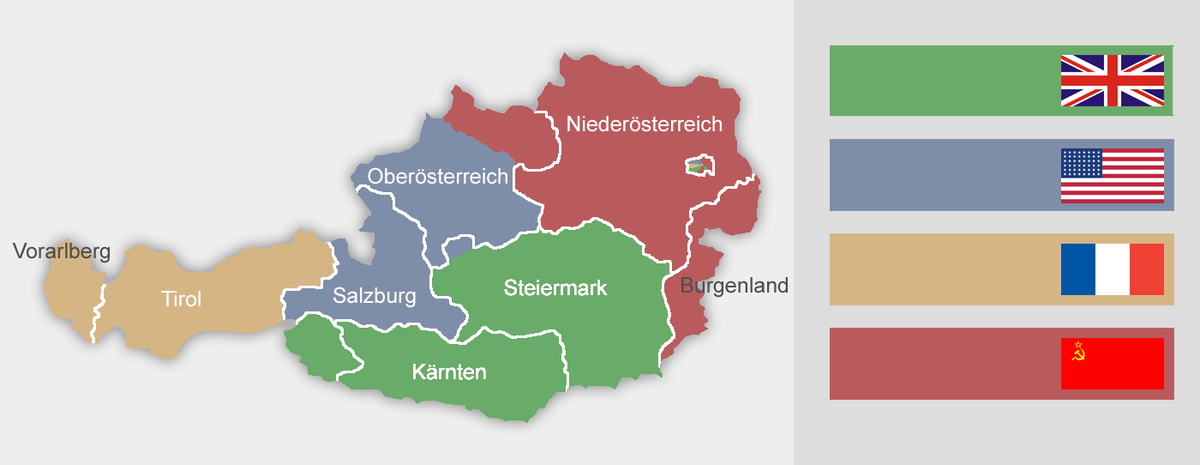
\includegraphics[width=\linewidth]{images/okupacniZony.png}

\end{minipage}
	\subsection*{První svobodné volby}
	25. listopadu 1945 se uskutečnily parlamentní volby. ÖVP (Österreichische Volkspartei, Rakouská lidová strana) získala 49,8\%, SPÖ (Sozialdemokratische Partei Österreichs, Sociálně demokratická strana Rakouska) 44,6\% a KPÖ (Kommunistische Partei Österreichs, komunisté) získali 5,4\%. ÖVP a SPÖ vytvořili koalici a komunisté přišli o podporu ve vládě. Komunisté však stále ovládaly značné množstní odborů.
	\subsection*{Hospodářská situace okolo roku 1950}
	Roku 1947 přijala vláda dohodu o~msdách a cenách, která začala vzbuzovat napětí. Tato situace byla vyřešena o~rok pozdějí přijetím Marshallova plánu. Roku 1950 dochází k~pozastavení Marshallova plánu díky americké válce s~Koreou. Toho využili komunisté a pokusili se vyvolat povstání. 4. října došlo k~rozsáhlým nepokojím ve východním rakousku všetně Vídně. Vláda zareagovala rychle avšak nepoužila pouze vojenskou sílu, ale i odbory. Tím zklidnili napětí a podařilo se jim situaci stabilizovat.
	\subsection*{Rakouské vyjednávání o nezávislosti}
	Od Stalinovy smrti se silně prosazuje myšlenka rakouské suverenity. Avšak ruští politici v čele s~Molotovem se staví proti a podmiňují neutralitu Rakouska vyřešením situace v~Německu. \par
	Roku 1955 začínalo být zjevné, že západní Německo se připojí k~NATO. Tudíž se dalo předpokládat, že pokud Rakousko nedostane suverenitu, tak se jeho západní čast rovněž stane součástí NATO. Což SSSR nevzhovovalo, neboť plánovali vytvořit \uv{neutrální} úzení (Rakousko, Jugoslávie, \dots). Tato skutečnost měla za následek, že Motolov odvolal  podmíněnost rakouské neutrality vyřešením Německého problému. Požadovali však aby si rakoský stát zachoval neutralitu vůči USA a zakazovali spojení Rakouska s Německem. Nakonec byla 15. května podepsána Rakouská státní smlouva, ve vídeňském zámku Belvedere která zaručovala Rakouskou suverenitu.
\end{minipage}
\hspace{0.5cm}
\begin{minipage}[t]{0.25\linewidth}
\Large
\renewcommand\arraystretch{1.4}\arrayrulecolor{LightSteelBlue3}
\captionsetup{singlelinecheck=false, font=blue, labelfont=sc, labelsep=quad}
\captionof*{table}{\huge Časová osa}\vskip -1.5ex
%\caption{Timeline}\vskip -1.5ex
\begin{tabular}{@{\,}r <{\hskip 2pt} !{\foo} >{\raggedright\arraybackslash}p{5cm}}
\toprule
\addlinespace[1.5ex]
červenec 1945 & vytvoření okupačních zón\\
listopad 1945 & první svobodné volby\\
1948 & přijetí Marshallova plánu\\
říjen 1950 & povstání z~důvodu ekonomiky\\
březen 1953 & úmrtí Stalina\\
květen 1955 & nabytí nezávislosti\\
\end{tabular}
\end{minipage}
\end{minipage}
\end{landscape}
\end{document}